% ===================== shared body for single- and double-column versions =====================
\title{A Policy-Conditioned Multi-Agent LLM Framework for Auditable, Evidence-Driven Trading Decision Support}

\author{\IEEEauthorblockN{Malhar Inamdar}
\IEEEauthorblockA{\textit{Dept. of Electronics \& Telecomm. Engg.}\\
\textit{Pune Institute of Computer Technology}\\
Pune, India\\
malhar.inamdar.097@gmail.com}
\and
\IEEEauthorblockN{Omkar Joshi}
\IEEEauthorblockA{\textit{Dept. of Electronics \& Telecomm. Engg.}\\
\textit{Pune Institute of Computer Technology}\\
Pune, India}
\and
\IEEEauthorblockN{Piyush Ochani}
\IEEEauthorblockA{\textit{Dept. of Electronics \& Telecomm. Engg.}\\
\textit{Pune Institute of Computer Technology}\\
Pune, India}
\and
\IEEEauthorblockN{Dr. P. S. Varade}
\IEEEauthorblockA{\textit{Dept. of Electronics \& Telecomm. Engg.}\\
\textit{Pune Institute of Computer Technology}\\
Pune, India}}

\maketitle

% ---------------------------------------------------------------- abstract
\begin{abstract}
Large language model (LLM) agents are increasingly used for financial analysis and trading, but three questions remain open: does such a system actually change its behaviour when the investor's mandate changes, is the confidence it reports trustworthy, and can it judge for itself how much evidence is enough before acting? This work develops a policy-conditioned, multi-agent framework in which a planner interprets an explicit, machine-readable investor policy that governs which specialist agents are consulted, how positions are sized, and when to stop gathering evidence, together with a deterministic risk engine that can veto any decision. Instead of claiming market-beating returns, the work evaluates the agent system itself. On live data for 40 US and Indian (NSE) stocks, one evidence bundle per stock was replayed under four investor profiles and three decision modes (480 decisions). When the LLM proposed its own trades and was shown the policy's numeric limits it broke none of them, but when it was given only a natural-language description of the same investor it broke the intended limits in 64.4\% of decisions (95\% CI 56.9--71.9\%) and in 98\% of the trades it made, proposing an average position of 11.5\% for a conservative profile capped at 2\%. Numeric baseline signals evaluated over three years showed no predictive edge and over-confident stated confidence (expected calibration error 0.071, reduced to 0.025 by temperature scaling). The results support machine-readable mandates with deterministic enforcement, and motivate measuring whether such enforcement improves realised outcomes.
\end{abstract}

\begin{IEEEkeywords}
Large language models, multi-agent systems, algorithmic trading, investor policy, AI governance, confidence calibration, decision support, auditability.
\end{IEEEkeywords}

% ---------------------------------------------------------------- 1 introduction
\section{Introduction}
LLM-based trading agents have progressed from single-prompt pipelines to full multi-agent systems and commercial products. However, the field's usual claim of higher returns in backtests has become hard to trust, since recent studies show such results are often inflated when the test period overlaps the model's training data \cite{gao2025lookahead,glasserman2024lookahead,alphaillusion}. At the same time, real investment decisions always depend on the investor's mandate: the same market evidence should lead a cautious long-term investor and an aggressive short-term trader to different actions. Existing systems rarely treat this mandate as a direct, machine-readable input, and few measure whether the system actually follows it. This project therefore shifts the focus from the market to the agent system itself, studying how controllable, trustworthy, and efficient it is, so that the contributions stay meaningful regardless of short-term profitability while still producing a complete working platform.

The closest work falls into three groups. Return-seeking agent teams such as TradingAgents \cite{tradingagents} and FinCon \cite{fincon} organise LLMs as analysts, researchers, traders, and risk managers, but evaluate them by cumulative return and Sharpe ratio. Studies of mandate behaviour show that an assigned investor profile can drift over a long simulation \cite{finpersona} and that risk profiles change portfolio allocations \cite{portbench}. Most recently, governance-oriented systems place a deterministic layer between the LLM and the market: OpenPM compiles natural-language mandates into enforced constraints \cite{openpm}, CLQT audits closed-loop portfolio agents \cite{clqt}, BiasMix-Finance reports that 47.6--85.7\% of raw LLM portfolio proposals violate the investor's caps before a projection step repairs them \cite{biasmix}, and Policy-as-Skill counts how often a deterministic controller overrides an LLM in compliance tasks \cite{policyasskill}. The architecture is therefore established; our work uses it as an instrument. What it adds is a controlled comparison on real US and Indian evidence: the same frozen evidence is replayed under several investor policies, the LLM is allowed to break the policy, and the deterministic layer's interventions are counted. None of the surveyed papers uses Indian market data.

The contributions of this work are:
\begin{itemize}
\item a machine-readable investor-policy format that governs evidence order, evidence budget, confidence threshold, position size, and stop-loss;
\item a working multi-agent decision-support system (LangGraph planner, four LLM agents, an ML predictor, volatility-target sizing, a deterministic risk engine, and an audit log) on live US and NSE data;
\item an evaluation suite that replays identical frozen evidence under every policy and three decision modes, measuring rule-following, deterministic-layer interventions, confidence calibration, and evidence cost;
\item a first experiment on \ObStocks{} US and NSE stocks: the LLM obeyed numeric policy limits in every decision (\ObExplicit{} violations), but given only a text profile it broke the intended limits in \ObNL{} of decisions (\ObNLacted{} of the trades it made).
\end{itemize}

The rest of the paper is organised as follows. Section~II surveys 32 related papers, Section~III states the problem and objectives, Sections~IV--VI describe the system, algorithm, and evaluation parameters, Section~VII the implementation, Section~VIII the results, and Section~IX concludes.

% ---------------------------------------------------------------- 2 literature survey
\section{Literature Survey}
Tables~\ref{tab:survey} and~\ref{tab:survey2} summarise the approach, data, and reported result of the 32 surveyed papers, grouped into five areas.

\subsection{LLM Agent Systems for Trading}
TradingAgents \cite{tradingagents} models a trading firm with fundamental, sentiment, news, and technical analysts, a bull--bear research debate, a trader, and a risk-management team, and reports at least 23.21\% cumulative return on three US technology stocks over January--March 2024. FinCon \cite{fincon} arranges a manager and analysts in a hierarchy and updates their beliefs through conceptual verbal reinforcement, reporting a cumulative return above 57\% with a Sharpe ratio of 0.825 on COIN. FinMem \cite{finmem} adds a layered memory and a configurable character profile and reports 61.78\% cumulative return on TSLA against $-18.63\%$ for buy-and-hold. FinAgent \cite{finagent} is a multimodal agent that reads news, prices, and candlestick charts with dual-level reflection, reporting over 36\% average profit improvement. FinRobot \cite{finrobot} provides an open four-layer platform, and MarketSenseAI \cite{marketsenseai} uses GPT-4 chain-of-thought stock selection with reported excess alpha of 10--30\% on S\&P 100 stocks. A recent survey \cite{llmtradingsurvey} catalogues these architectures. \emph{Observation:} all of these systems are judged mainly by returns over short, single-market windows, and none tests whether an investor's stated limits are respected.

\subsection{Financial Language Models and Reinforcement Learning}
BloombergGPT \cite{bloomberggpt} trains a 50-billion-parameter model on 363 billion financial tokens and reports an average of 62.51 on public financial tasks against 51.90 for GPT-NeoX. FinGPT \cite{fingpt} takes an open, data-centric route with automatic data curation and low-rank fine-tuning, and FinRL \cite{finrl} offers deep reinforcement learning agents for trading on US, Chinese, and Hong Kong indices. \emph{Observation:} these works improve the model or the learner, whereas our system keeps a general LLM and controls its behaviour through an explicit policy and a deterministic layer.

\subsection{Evaluation Benchmarks and Look-Ahead Bias}
Because LLMs may have seen historical prices and news during training, several works question backtested results. Glasserman and Lin \cite{glasserman2024lookahead} show that anonymising firm names in headlines changes in-sample performance by 5.89 basis points per day, and Gao et al. \cite{gao2025lookahead} propose a look-ahead propensity statistic that falls to near zero after a model's training cutoff. The Alpha Illusion \cite{alphaillusion} argues that reported alpha should not be taken as deployment evidence and finds that realistic frictions cut a TradingAgents portfolio Sharpe ratio from 0.43 to 0.22. Contamination-free benchmarks such as StockBench \cite{stockbench} (Dow Jones stocks, March--June 2025, best agent 1.9\% return against 0.4\% for buy-and-hold) and Agent Market Arena \cite{agentmarketarena} (live trading of stocks and cryptocurrencies) still rank agents by profit. Newer benchmarks evaluate the decision process: CLQT \cite{clqt} measures a gap between what an agent says and what it does, PortBench \cite{portbench} finds that only 32.5\% of 120 LLM allocations beat equal weighting on Sharpe ratio, OpenPM \cite{openpm} finds that GPT-5's edge over an equal-weight portfolio of the same stocks is only 2.1--2.9 percentage points under point-in-time evaluation, InvestLogicBench \cite{investlogicbench} scores reasoning traces of real investors, and KTD-Fin \cite{ktdfin} measures order-level confidence on Chinese CSI300 stocks. \emph{Observation:} careful evaluation repeatedly shrinks or removes the returns that agent papers report, which supports measuring behaviour rather than profit.

\subsection{Investor Mandates, Personas, and Governance}
FinPersona-Bench \cite{finpersona} measures how an assigned mandate loses influence over a long synthetic-market simulation across 18 LLMs; in crash scenarios the behaviour gap between static and periodically re-grounded agents grows 4.4 times. Persona-collapse analysis \cite{personacollapse} finds that three frontier models put over 90\% of financial-advice responses into a single persona. BiasMix-Finance \cite{biasmix}, accepted at the ICLR 2026 Financial AI workshop, finds that 47.6--85.7\% of first-pass LLM portfolios break investor caps and repairs them to 0\% with a convex projection. ReguSim \cite{regusim} shows that even with the rules visible, 14.8--24.2\% of LLM orders are rejected by a compliance simulator, and ActionAudit \cite{actionaudit} scores advice against a replayable deterministic baseline. Policy-as-Skill \cite{policyasskill} packages organisational policy as versioned executable skills with audit trails, and finds that its deterministic controller changes 66.8\% of decisions, helping some task types and hurting others. \emph{Observation:} raw LLM decisions often ignore stated constraints, and deterministic enforcement fixes feasibility; however, none of these works measures whether the enforced decisions lead to better realised outcomes, and none uses Indian market data.

\subsection{Calibration, Agents, and Backtest Statistics}
Guo et al. \cite{guo2017calibration} show that modern neural networks are over-confident and that temperature scaling reduces expected calibration error, for example from 16.53\% to 1.26\% on CIFAR-100. Xiong et al. \cite{xiong2024confidence} find that LLMs' verbalised confidence is also over-confident. In finance, KTD-Fin \cite{ktdfin} reports order-confidence calibration errors of 0.246--0.425 across ten LLMs, and Ordinal Gates \cite{ordinalgates} shows that fixed confidence thresholds gave no significant gain in 18 configurations, because LLM confidence carries little information about correctness. ReAct \cite{react} provides the reason-then-act pattern used by our agents, while Bailey and L\'opez de Prado \cite{bailey2014deflated} and L\'opez de Prado \cite{lopezdeprado2018} give the deflated Sharpe ratio and purged cross-validation needed before any performance claim.

\subsection{Observations and Research Gap}
Fig.~\ref{fig:surveychart} counts what the 32 surveyed papers actually measure. Returns (17 papers) and risk metrics (21) dominate; rule or mandate following is measured by 9, look-ahead leakage is controlled by 12, cost by 12, confidence calibration by only 4, and Indian market data by none. Three gaps follow: (i) when a deterministic layer overrides an LLM trading decision, whether the outcome improves or worsens has not been measured; (ii) investor policies are rarely compared on identical evidence, with the LLM free to violate them; and (iii) no leakage-aware LLM trading study covers NSE stocks. This work builds the system and the evaluation suite for these questions and reports the first experiments.

\SurveyTable

\begin{figure}[!htbp]
\centering
\IfFileExists{figs/fig_survey_coverage.png}{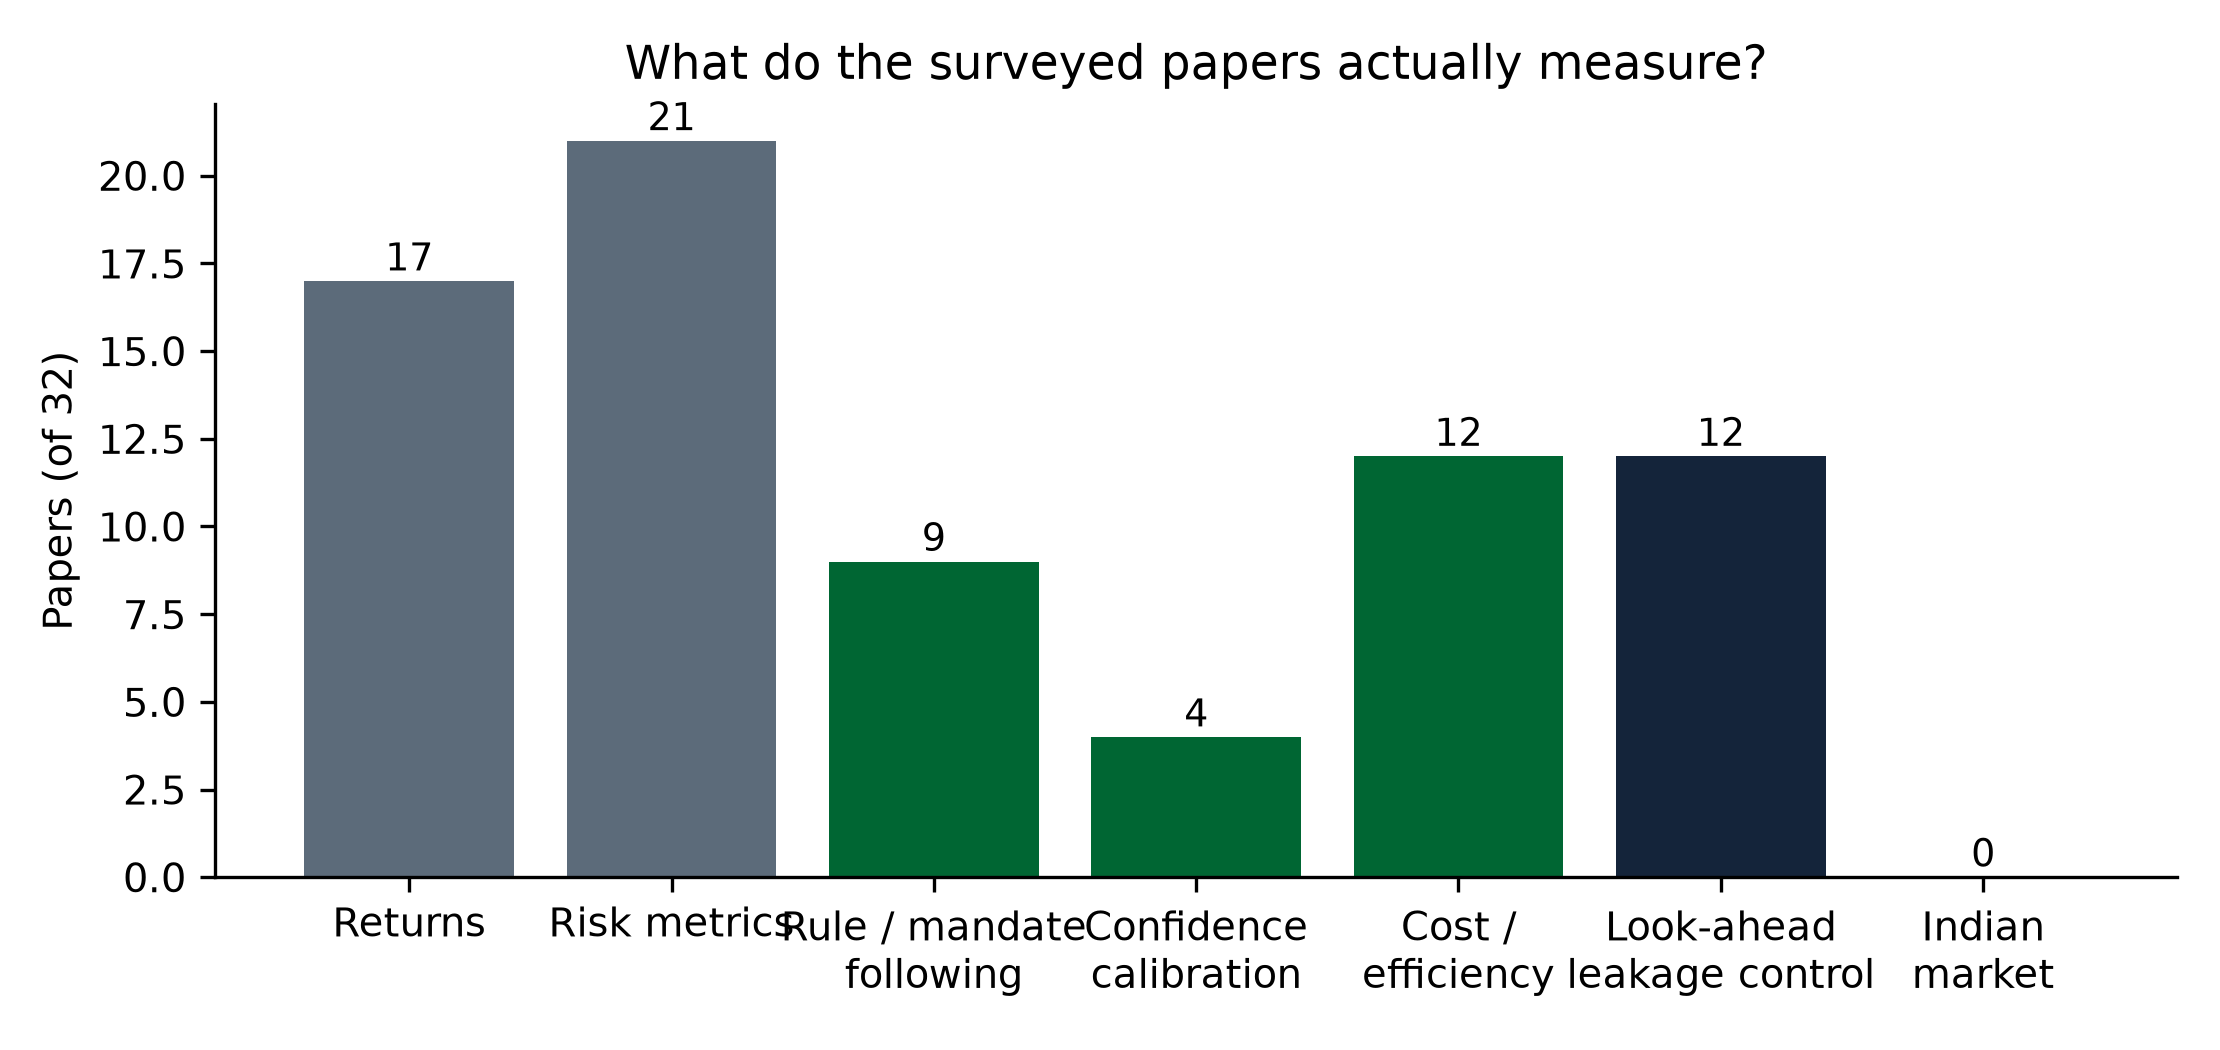
\includegraphics[width=\figW]{figs/fig_survey_coverage.png}}{}
\caption{Number of surveyed papers (out of 32) that evaluate each property. Profit and risk are widely measured; rule following, confidence calibration, and Indian-market data are rarely measured.}
\label{fig:surveychart}
\end{figure}

% ---------------------------------------------------------------- 3 problem
\section{Problem Definition and Objectives}
\textbf{Problem statement.} To build a multi-agent LLM trading system whose behaviour is governed by an explicit investor policy under a rule-based risk check, and to evaluate how faithfully it follows that policy, how reliable its confidence is, and how efficiently it uses evidence, using paper trading on US and Indian equities.

\textbf{Objectives.}
\begin{enumerate}
\item Design an investor-policy format and a policy-driven planner, and build the supporting pipeline of data ingestion, specialist agents, ML tools, a rule-based risk engine, and paper-trading execution.
\item Evaluate how faithfully the system follows different investor policies when given the same market evidence.
\item Assess the reliability of the system's confidence and the trade-off between decision quality and the cost of gathering evidence.
\item Validate the system through paper trading on US and Indian equities, treating financial returns as secondary indicators.
\end{enumerate}

% ---------------------------------------------------------------- 4 proposed system
\section{Proposed System}
The system has five main parts (Fig.~\ref{fig:block}): a data pipeline that collects and prepares market prices, news, and economic indicators; a policy-conditioned planner that reads the active investor policy and decides which specialist agents and tools to use, how much evidence to gather, and how to size a position; a set of LLM specialist agents (technical, news, fundamental, and macro) supported by a classical machine-learning model for numeric predictions; a deterministic rule-based risk engine that can veto any trade and is deliberately kept free of AI so its safety limits stay transparent and auditable; and a paper-trading execution and logging layer. Every decision is recorded together with the evidence and policy rules behind it, which keeps the system auditable and supports the evaluation; the same evidence can also be replayed under different policies to compare behaviour directly.

Each evidence source returns a direction between $-1$ (bearish) and $+1$ (bullish), a confidence between 0 and 1, a reliability weight, and the cost of producing it. The LLM agents only interpret evidence; position sizes, stop-losses, and indicator values always come from code. The four investor profiles used in this work are listed in Table~\ref{tab:policy}; they differ in position cap, stop-loss, confidence threshold, evidence budget, volatility budget, and the order in which evidence is consulted. The flowchart of one decision is shown in Fig.~\ref{fig:flow}.

\begin{figure*}[!t]
\centering
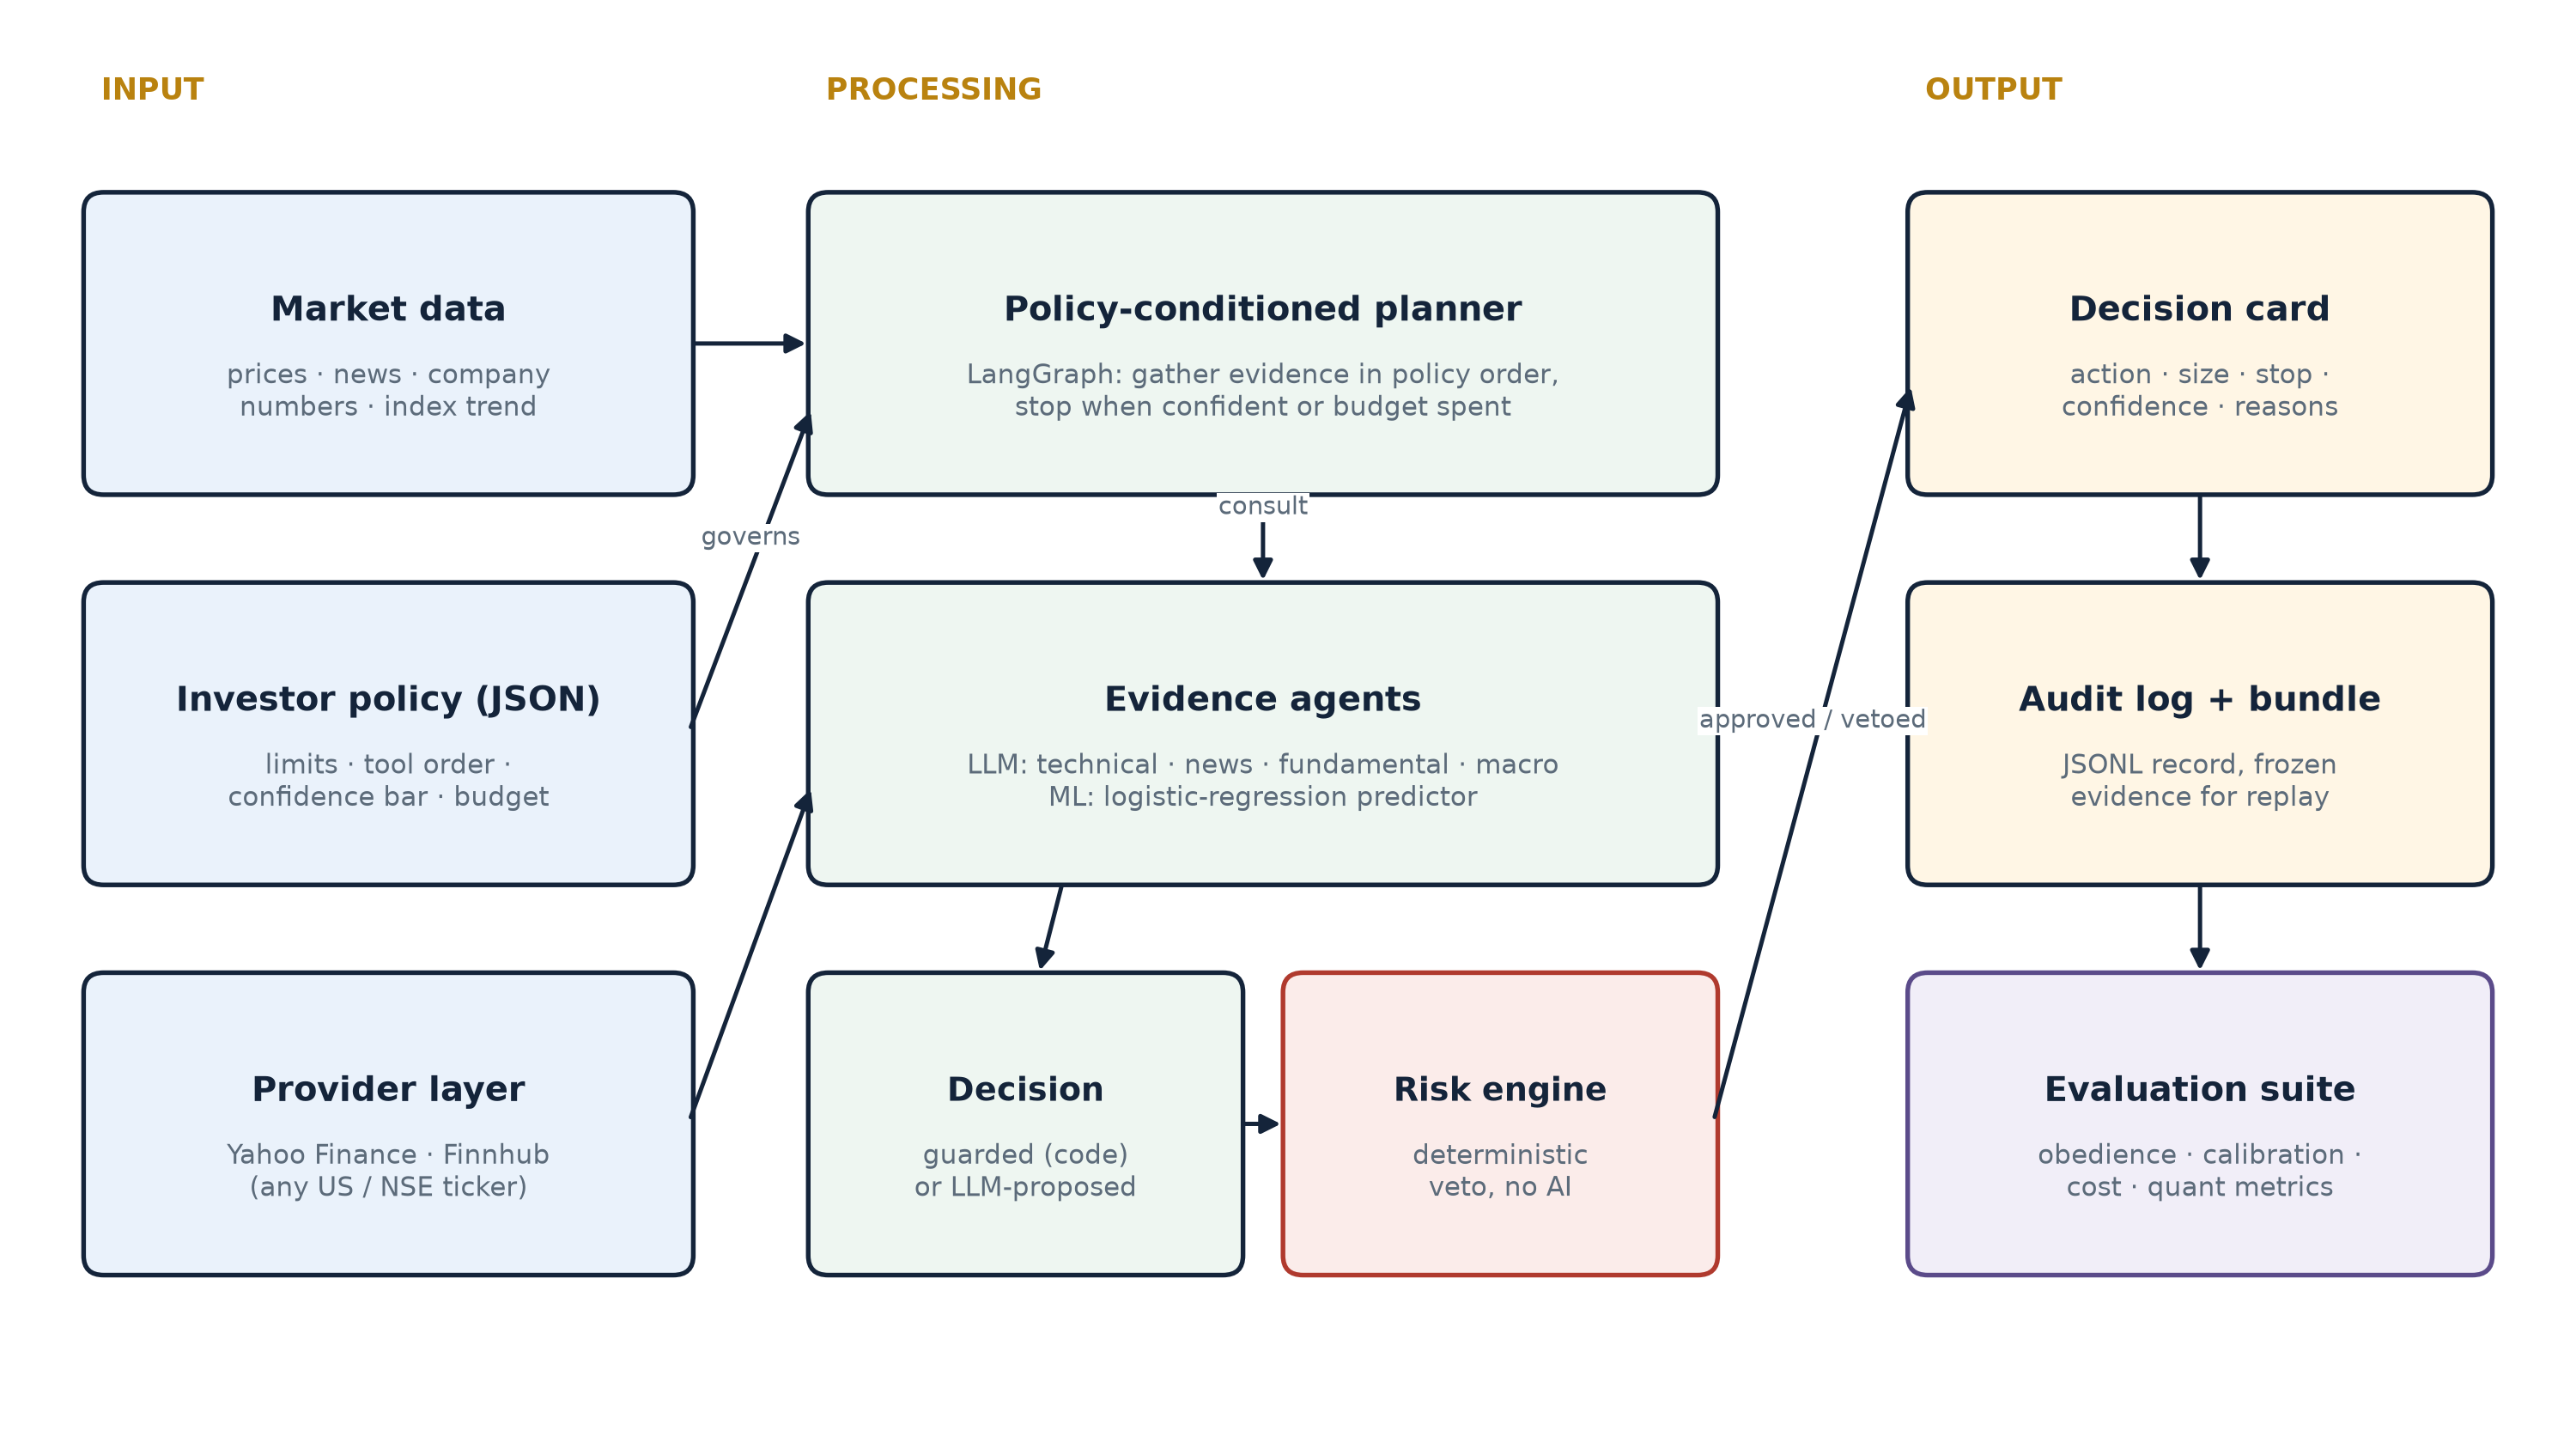
\includegraphics[width=0.9\textwidth]{figs/fig_block_diagram.png}
\caption{Proposed block diagram (input, processing, output). The investor policy governs the planner; the deterministic risk engine audits every decision before it is logged.}
\label{fig:block}
\end{figure*}

\PolicyTable

\begin{figure}[!htbp]
\centering
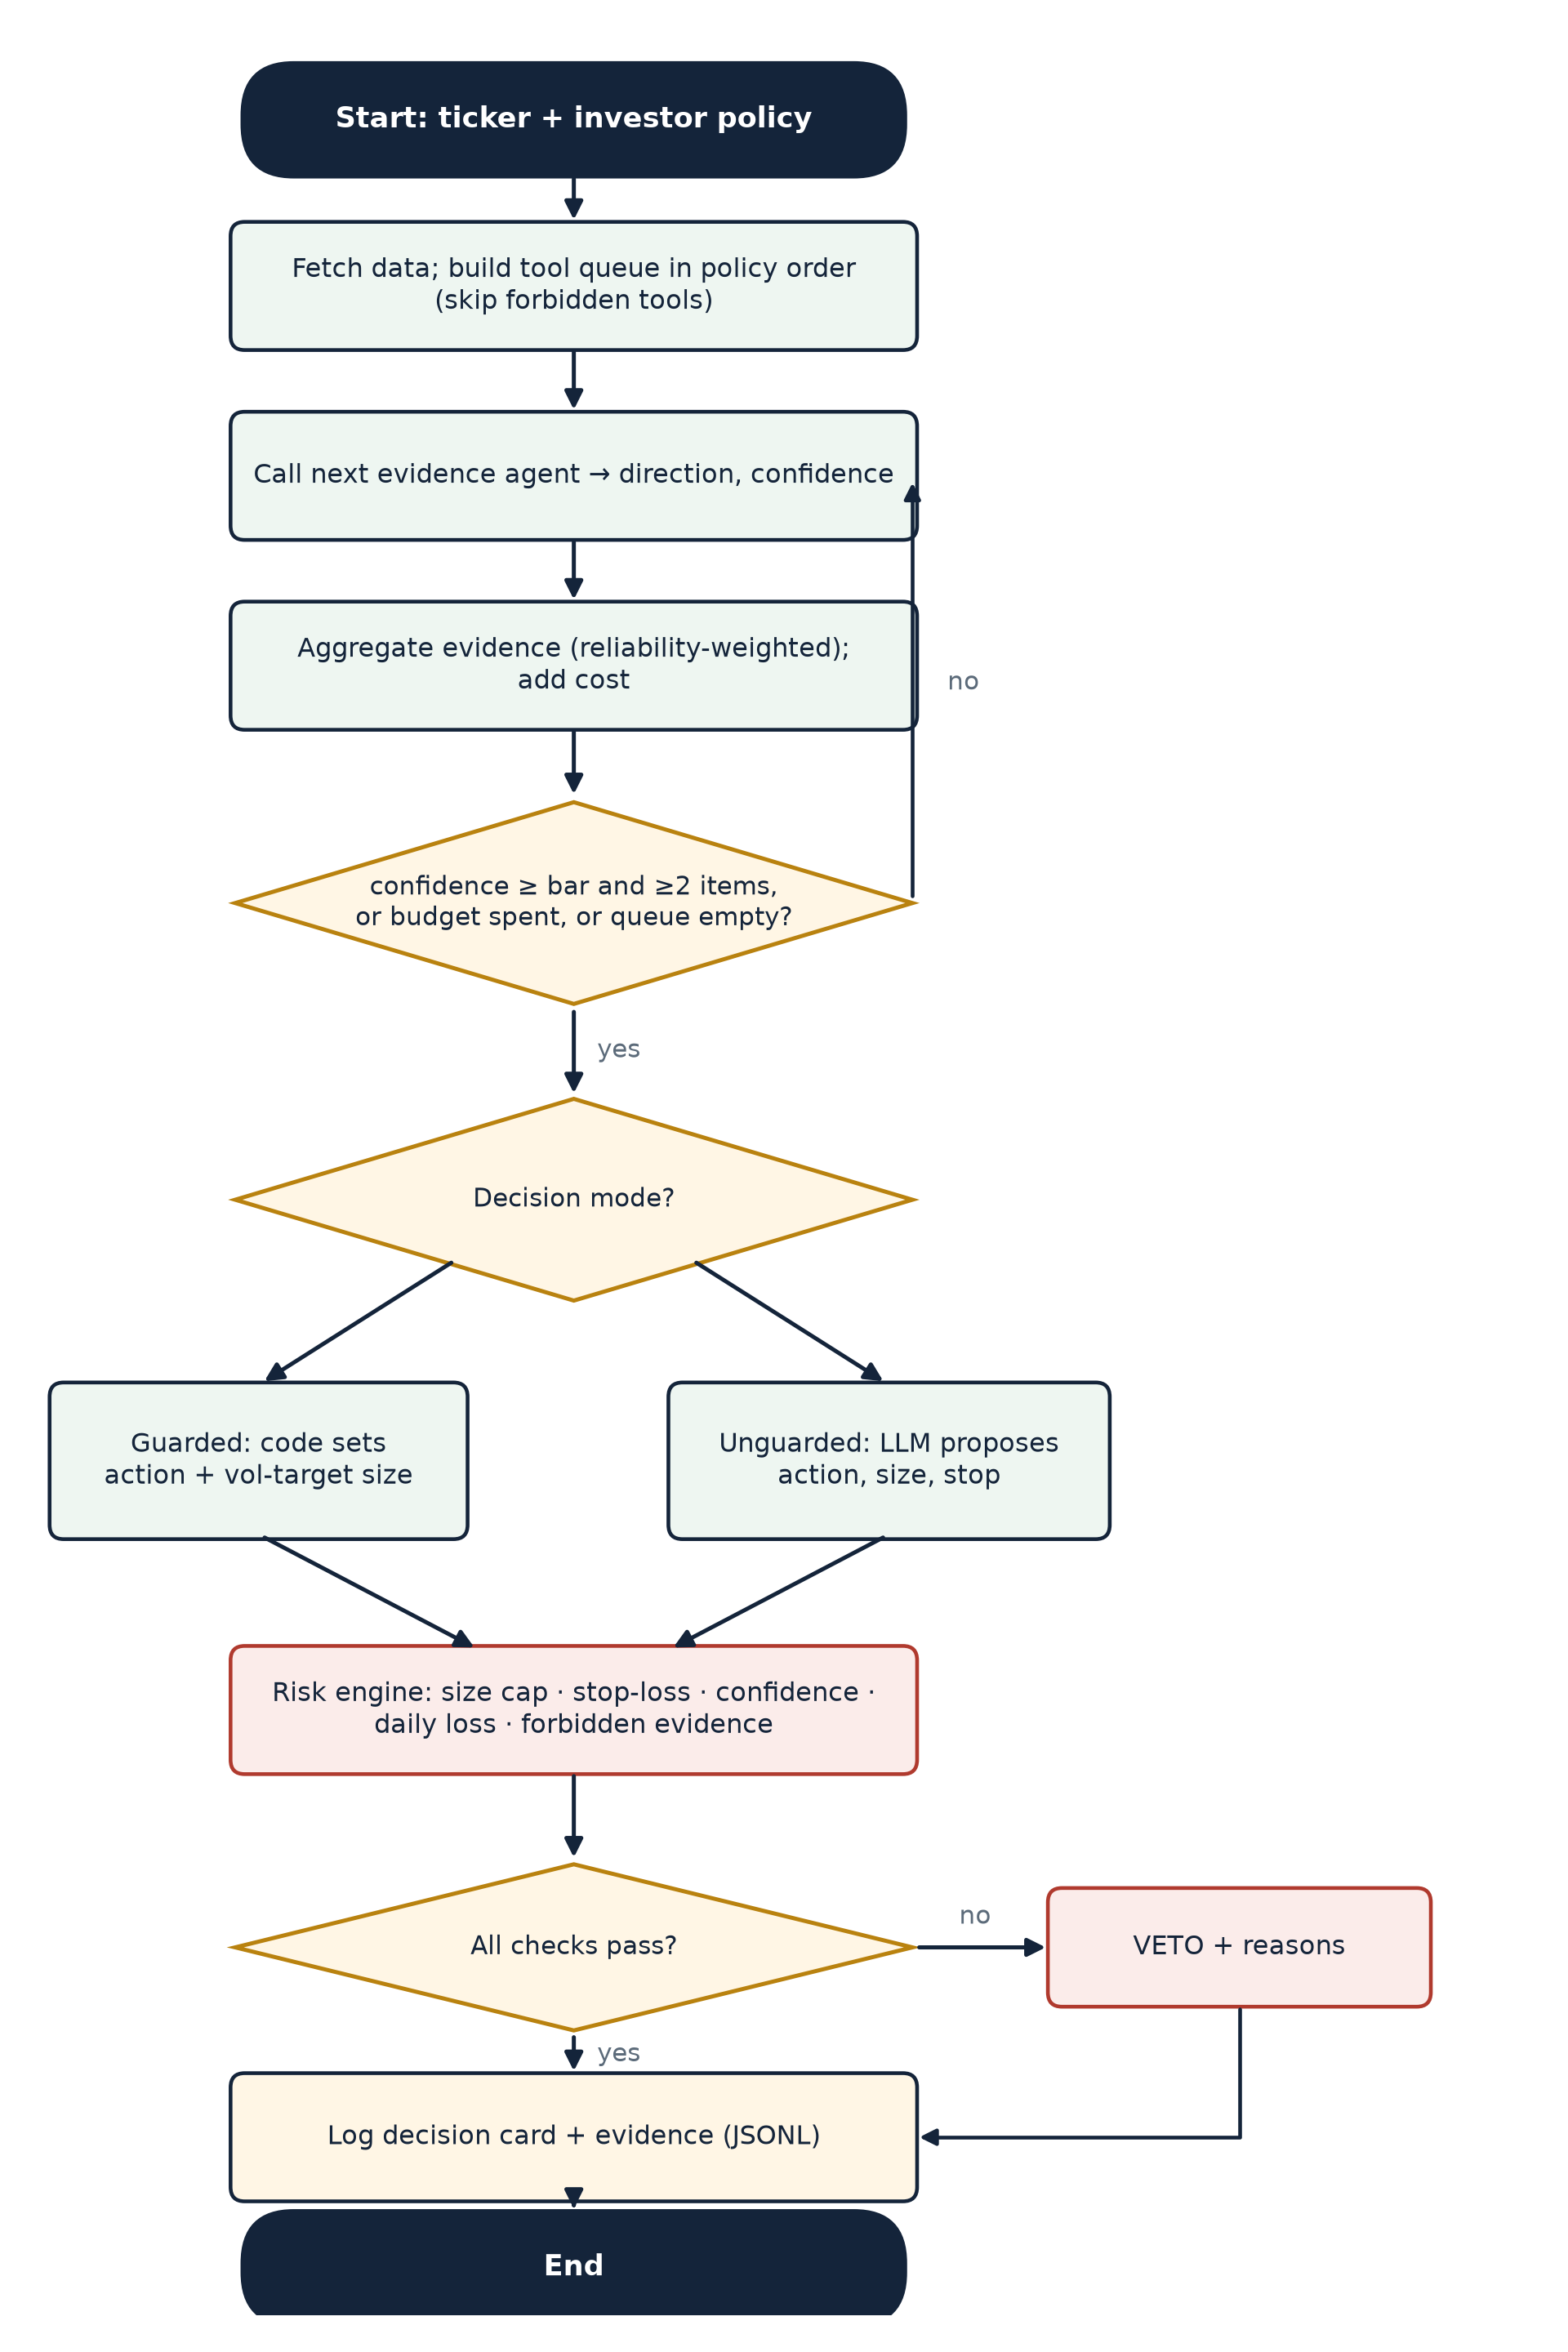
\includegraphics[width=\flowW]{figs/fig_flowchart.png}
\caption{Flowchart of one decision: policy-ordered evidence gathering with adaptive stopping, guarded or unguarded decision, and deterministic risk audit.}
\label{fig:flow}
\end{figure}

% ---------------------------------------------------------------- 5 algorithm
\section{Algorithm}
Algorithm~\ref{alg:decide} gives one decision. Evidence items carry a direction $d_k\in[-1,1]$, a confidence $c_k\in[0,1]$, a reliability weight $w_k$, and a cost $u_k$. The planner consults tools in the order fixed by the policy and skips any tool the policy forbids. After each tool it forms a reliability- and confidence-weighted direction $\bar d$ and confidence $\bar c$, reducing $\bar c$ by 20\% when the evidence disagrees in sign, and it stops as soon as the policy's confidence threshold is reached with at least two items or the evidence budget is spent. In the guarded mode the action and size are then computed in code; in the two unguarded modes the LLM proposes them. In every mode the same risk engine checks the result.

\begin{algorithm}[!htbp]
\caption{Policy-conditioned decision with deterministic audit}
\label{alg:decide}
\begin{algorithmic}[1]
\Require ticker $x$, policy $\pi$, evidence tools $T$, mode $m$
\State $Q \gets$ tools of $\pi.\text{priorities}$ in order, excluding $\pi.\text{forbidden}$
\State $E \gets \emptyset$;\; $C \gets 0$
\While{$Q \neq \emptyset$ \textbf{and} $C < \pi.\text{budget}$}
  \State $(d,c,w,u) \gets$ \Call{CallTool}{$Q.\text{pop}(), x$};\; $E \gets E \cup \{(d,c,w)\}$;\; $C \gets C + u$
  \State $\bar d \gets \frac{\sum_k w_k c_k d_k}{\sum_k w_k c_k}$;\; $\bar c \gets \frac{\sum_k w_k c_k}{\sum_k w_k}$
  \If{signs of $d_k$ disagree} $\bar c \gets 0.8\,\bar c$ \EndIf
  \If{$\bar c \ge \pi.\text{conf}$ \textbf{and} $|E| \ge 2$} \textbf{break} \EndIf
\EndWhile
\If{$m = \text{guarded}$}
  \If{$\bar c < \pi.\text{conf}$ \textbf{or} $|\bar d| < 0.15$} $a \gets \text{WAIT}$, $s \gets 0$
  \Else
    \State $a \gets$ BUY if $\bar d>0$, else SELL
    \State $s \gets \min\!\big(\tfrac{\sigma^\ast}{\hat\sigma}\,|\bar d|\,\bar c,\ \pi.\text{max\_pos}\big)$;\; $\ell \gets \pi.\text{stop}$
  \EndIf
\Else
  \State $(a,s,\ell,\hat c) \gets$ LLM proposal given $E$ and the policy (numeric rules or text profile)
\EndIf
\State verdict $\gets$ \Call{RiskEngine}{$a,s,\ell,\hat c,\pi$} \Comment{size cap, stop-loss, confidence, daily loss, forbidden evidence}
\State \Return log$(x,\pi,m,a,s,\ell,E,\text{verdict})$
\end{algorithmic}
\end{algorithm}

Here $\sigma^\ast$ is the policy's per-position volatility budget and $\hat\sigma$ the stock's realised annual volatility, so a calmer stock receives a larger position than a volatile one for the same conviction.

% ---------------------------------------------------------------- 6 performance parameters
\section{Performance Evaluation Parameters}
For $N$ logged decisions, the violation rate of rule $r$ (position above cap, stop-loss missing or looser than the policy, acting below the confidence threshold) is
\begin{equation}
V_r=\frac{1}{N}\sum_{i=1}^{N}\mathbb{1}[\text{decision } i \text{ breaks rule } r],
\end{equation}
and the any-violation rate $V$ counts a decision once if it breaks any rule. The intervention rate $I$ is the share of decisions vetoed by the risk engine. For $M$ evidence bundles replayed under policies $P$, action divergence is
\begin{equation}
D=\frac{1}{M}\sum_{j=1}^{M}\mathbb{1}\big[\,|\{a_{j,p}: p\in P\}|>1\,\big].
\end{equation}
Calibration uses the expected calibration error over bins $B_b$ and the Brier score,
\begin{equation}
\text{ECE}=\sum_{b}\frac{|B_b|}{n}\big|\text{acc}(B_b)-\text{conf}(B_b)\big|,
\end{equation}
\begin{equation}
\text{BS}=\frac{1}{n}\sum_{i}(p_i-y_i)^2 .
\end{equation}
Signal quality is the information coefficient $\text{IC}=\operatorname{corr}(\hat s_t, r_{t+1})$ with $t=\text{IC}\sqrt{n-2}/\sqrt{1-\text{IC}^2}$; trading quality uses the annualised Sharpe ratio $\sqrt{252}\,\mu_r/\sigma_r$ and maximum drawdown; cost is the mean number of evidence units used per decision. Rule-following and returns are always reported separately so that a system cannot trade safety for profit inside one score.

% ---------------------------------------------------------------- 7 implementation
\section{Implementation}
The implementation stack is listed in Table~\ref{tab:stack}. Market data are fetched through a provider layer so that the agents never call a data source directly; prices and company figures come from Yahoo Finance, and news and fundamentals from Finnhub with Google News as a fallback. A company-name resolver maps names such as ``Reliance'' to the NSE symbol, so the system can analyse any listed US or Indian stock. The research universe is fixed in advance at 20 US and 20 NSE large-cap stocks. Each decision is written as one JSON line containing the action, size, stop-loss, confidence, every evidence item, the policy clauses applied, the evidence cost, and the risk verdict, and the evidence of each moment is frozen in a bundle that can be replayed under any policy. Nine automated tests check the core invariants, including deterministic replay and risk-engine vetoes.

\StackTable

\textbf{Experimental setup.} One evidence bundle per stock was gathered from live data on 4 October 2026 and stored with its volatility context. Each bundle was replayed under the four investor policies in three decision modes: \emph{guarded} (action and size computed in code from the policy), \emph{unguarded-explicit} (the LLM proposes action, size, and stop-loss and is shown the policy's numeric rules), and \emph{unguarded-text} (the LLM sees only the policy's objective and horizon as text, such as ``protect capital over weeks to months''). All decisions were audited by the same risk engine and logged unmodified, giving 480 decisions. The model was \texttt{gpt-4o-mini} at temperature 0. Numeric baselines were evaluated separately over three years of daily data with transaction and slippage costs.

% ---------------------------------------------------------------- 8 results
\section{Results and Discussion}
\subsection{Rule Following on Identical Evidence}
Table~\ref{tab:obedience} and Fig.~\ref{fig:viol} report how often each mode broke the investor policy. The guarded mode cannot break the policy because code sets the size, so it serves only as a reference. When the LLM proposed its own trades and was shown the numeric rules, none of its 160 decisions broke a limit: every trade it made sat exactly at the policy cap (2\%, 5\%, 4\%, and 8\%). It was, however, more cautious than the guarded mode, trading in 31\% of decisions against 48\%, and the conservative profile traded in only 8\% of cases. When the same LLM saw only a text description of the investor, it broke the intended limits in 64.4\% of decisions (95\% CI 56.9--71.9\%) and in 98\% of the trades it made. The risk engine vetoed 103 proposals; all of them were above the position cap, 51 also had a missing or looser stop-loss, and 9 were placed below the confidence threshold (Fig.~\ref{fig:clause}). The violation rate was higher for US stocks (70.0\%) than for NSE stocks (58.8\%).

\ObedienceTable

\begin{figure}[!htbp]
\centering
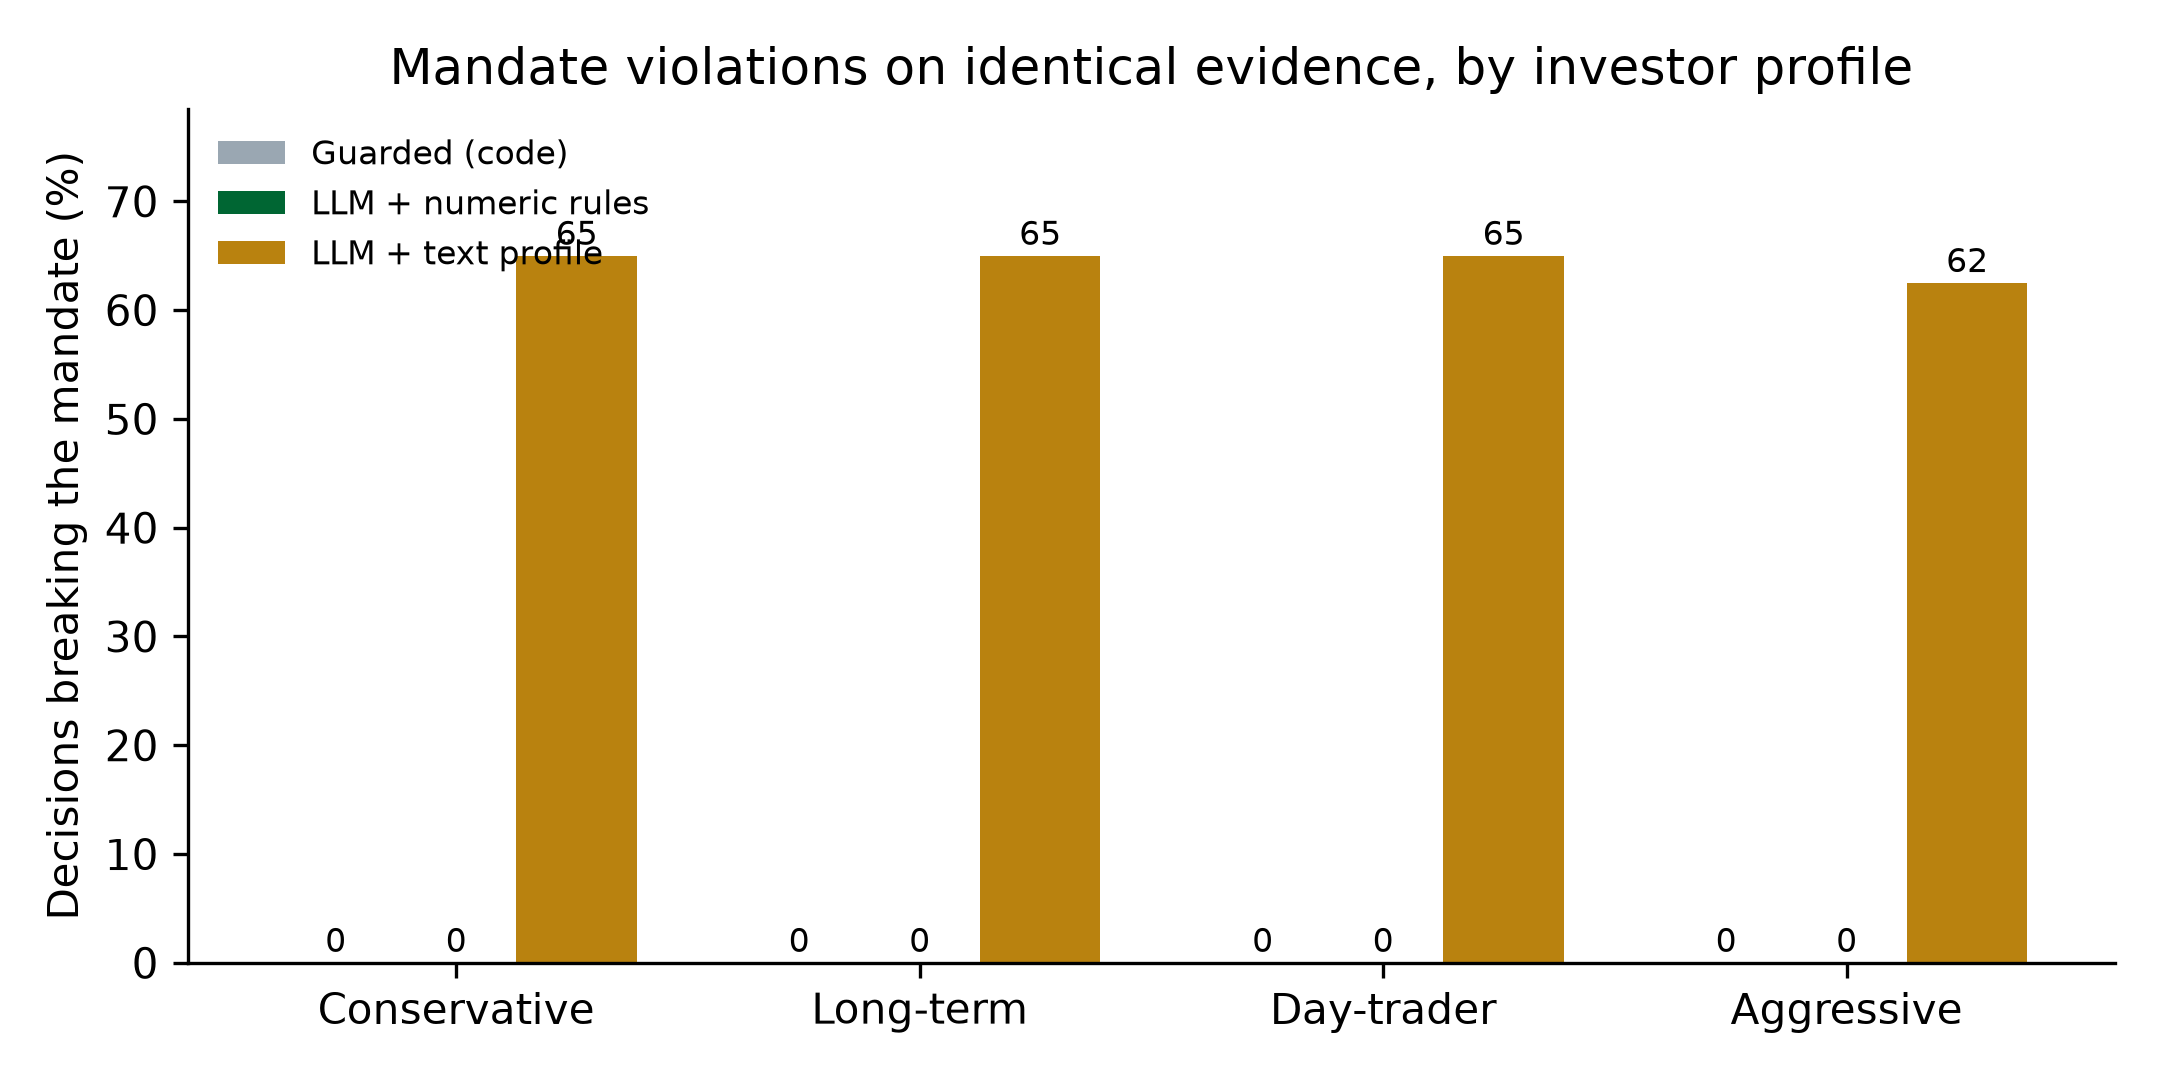
\includegraphics[width=\figW]{figs/fig_violations_by_profile.png}
\caption{Share of decisions breaking the investor policy on identical evidence, by profile and decision mode.}
\label{fig:viol}
\end{figure}

\begin{figure}[!htbp]
\centering
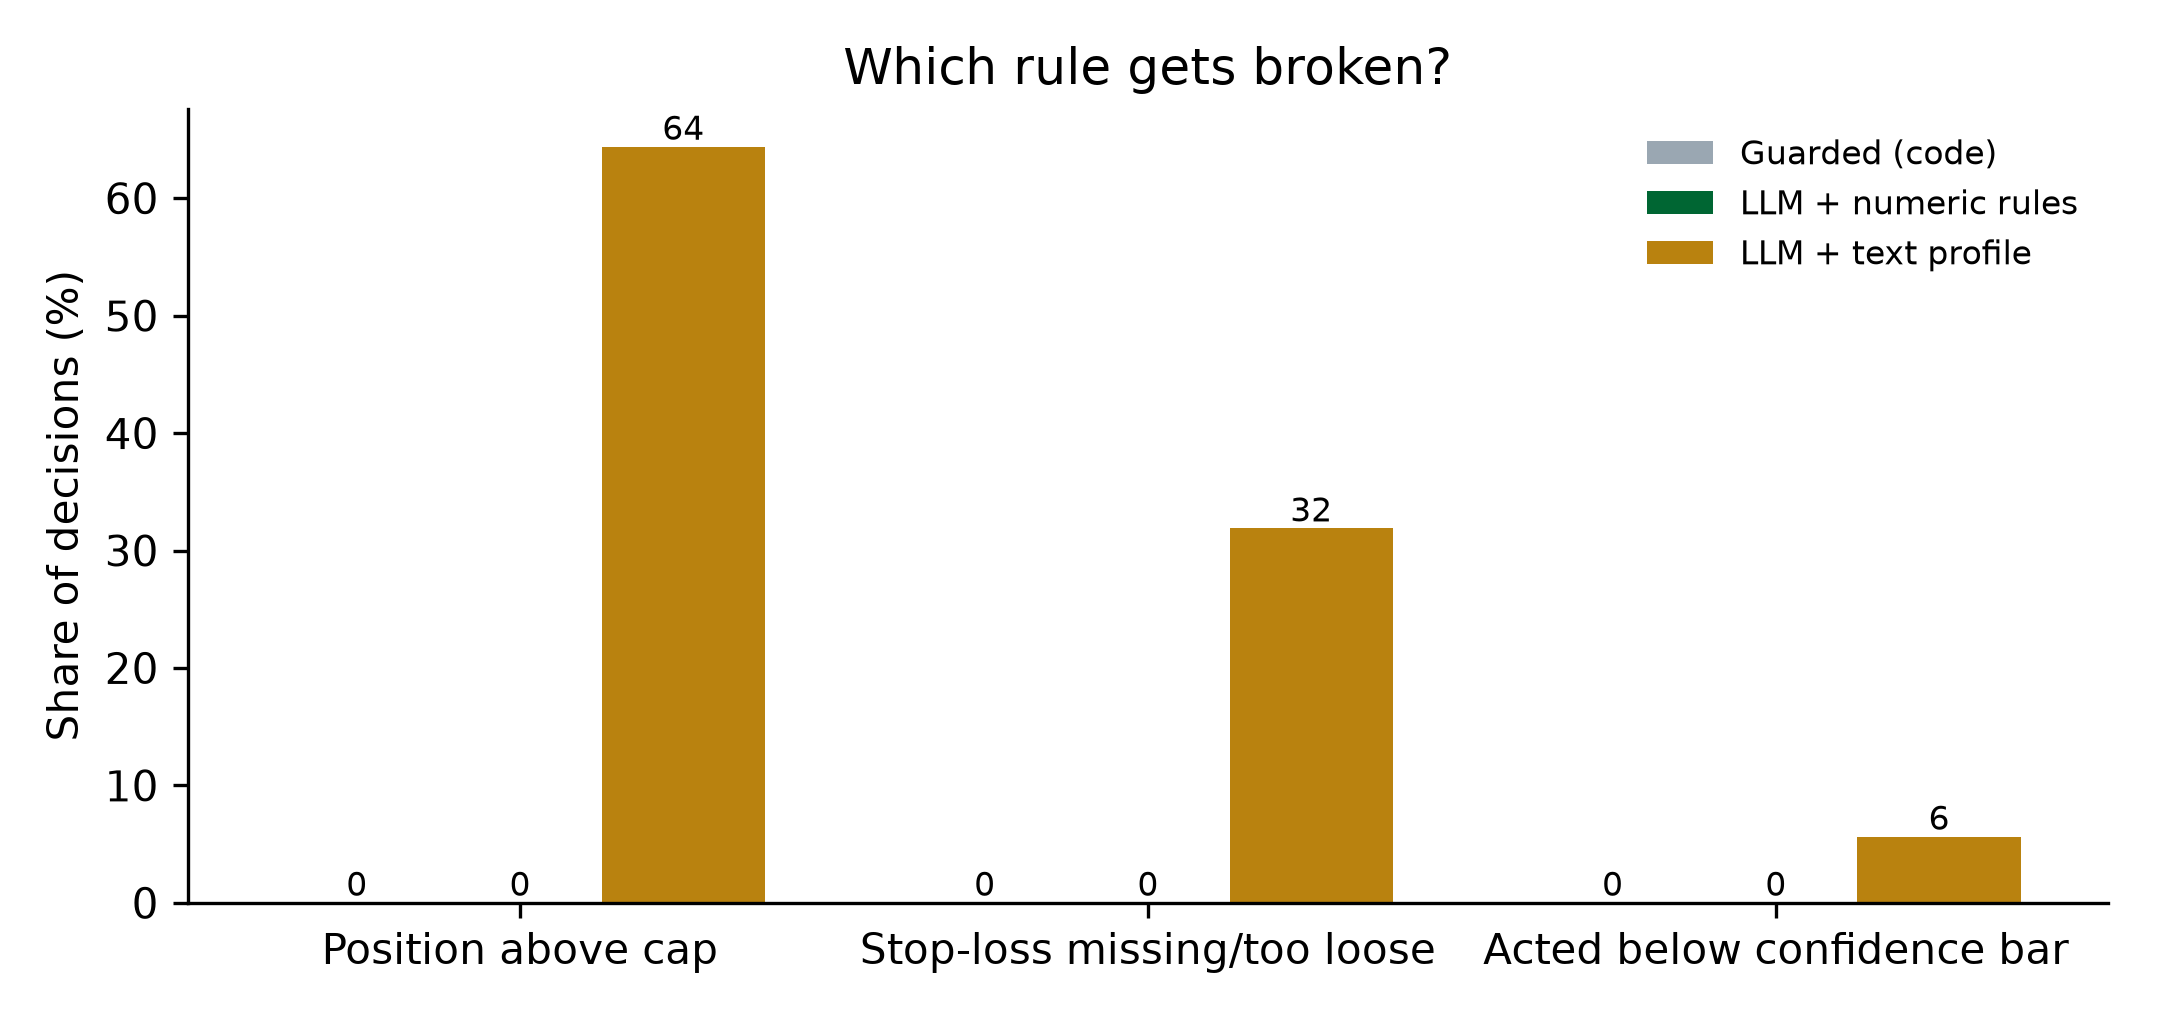
\includegraphics[width=\figW]{figs/fig_violations_by_clause.png}
\caption{Which rule is broken: position size above the cap dominates, followed by missing or loose stop-losses.}
\label{fig:clause}
\end{figure}

\subsection{Position Sizing Across Investor Profiles}
Fig.~\ref{fig:size} compares the mean proposed position size with each profile's cap. In the guarded and numeric-rule modes the sizes follow the profiles' risk ordering. In the text-only mode the LLM proposed 8--12\% positions for every profile, and the conservative profile received the largest average position (11.5\% against a 2\% cap), so the written description did not produce any risk ordering. Profiles still changed the decision on identical evidence: action labels differed across the four profiles on 78\% of stocks in the guarded mode, 70\% with numeric rules, and 80\% with the text profile. An important caveat is that in the text mode the numeric limits were never shown, so this result shows that a prose persona does not produce the limits an investor intends, rather than deliberate disobedience. It agrees with BiasMix-Finance \cite{biasmix} and supports expressing mandates in machine-readable form with deterministic enforcement.

\begin{figure}[!htbp]
\centering
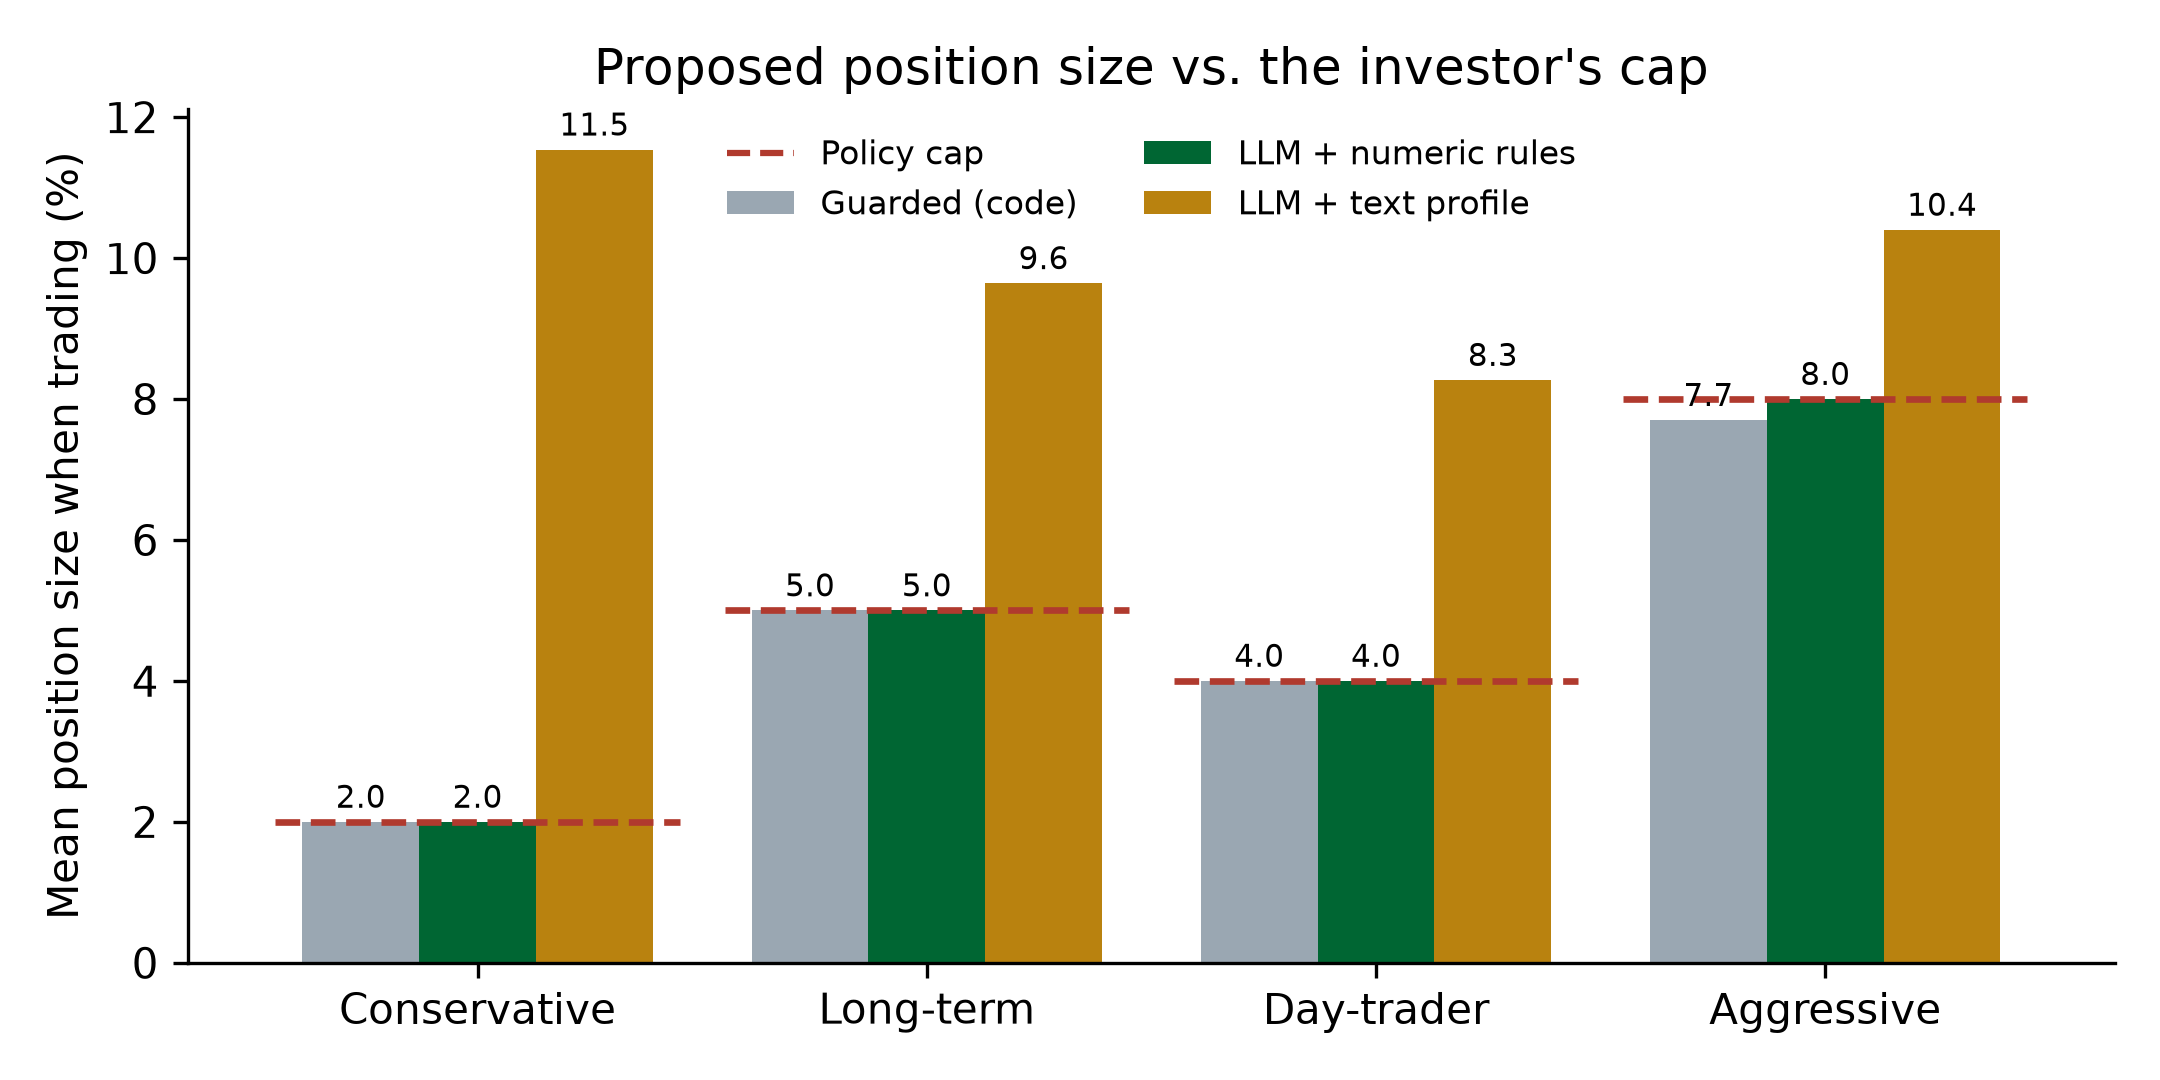
\includegraphics[width=\figW]{figs/fig_size_vs_cap.png}
\caption{Mean proposed position size when trading, against each profile's cap (dashed). With only a text profile the LLM proposed 8--12\% positions for every profile, including the conservative one (cap 2\%).}
\label{fig:size}
\end{figure}

\subsection{Numeric Baselines: Signal Quality, Calibration, and Evidence Cost}
Table~\ref{tab:baseline} reports the numeric baseline signals over three years of daily data. None of the four signals had a meaningful information coefficient (between $-0.027$ and $+0.030$), and none was significant on any stock. Their stated confidence was over-confident: calls made with about 73\% confidence were correct only about 52\% of the time (Fig.~\ref{fig:rel}), with an expected calibration error of 0.071 and a Brier score of 0.258. Temperature scaling reduced the calibration error to 0.025, but it did so by pulling all confidences toward 50\%, which is the correct response for a signal without predictive value. Gathering more evidence did not help either: as the stopping threshold was raised, the number of sources used rose from 2.0 to 2.9 while directional accuracy stayed at 50.1\% (Fig.~\ref{fig:cost}). These are baselines, not the LLM agents; they set the level that the agents must beat in the planned historical replay.

\begin{figure}[!htbp]
\centering
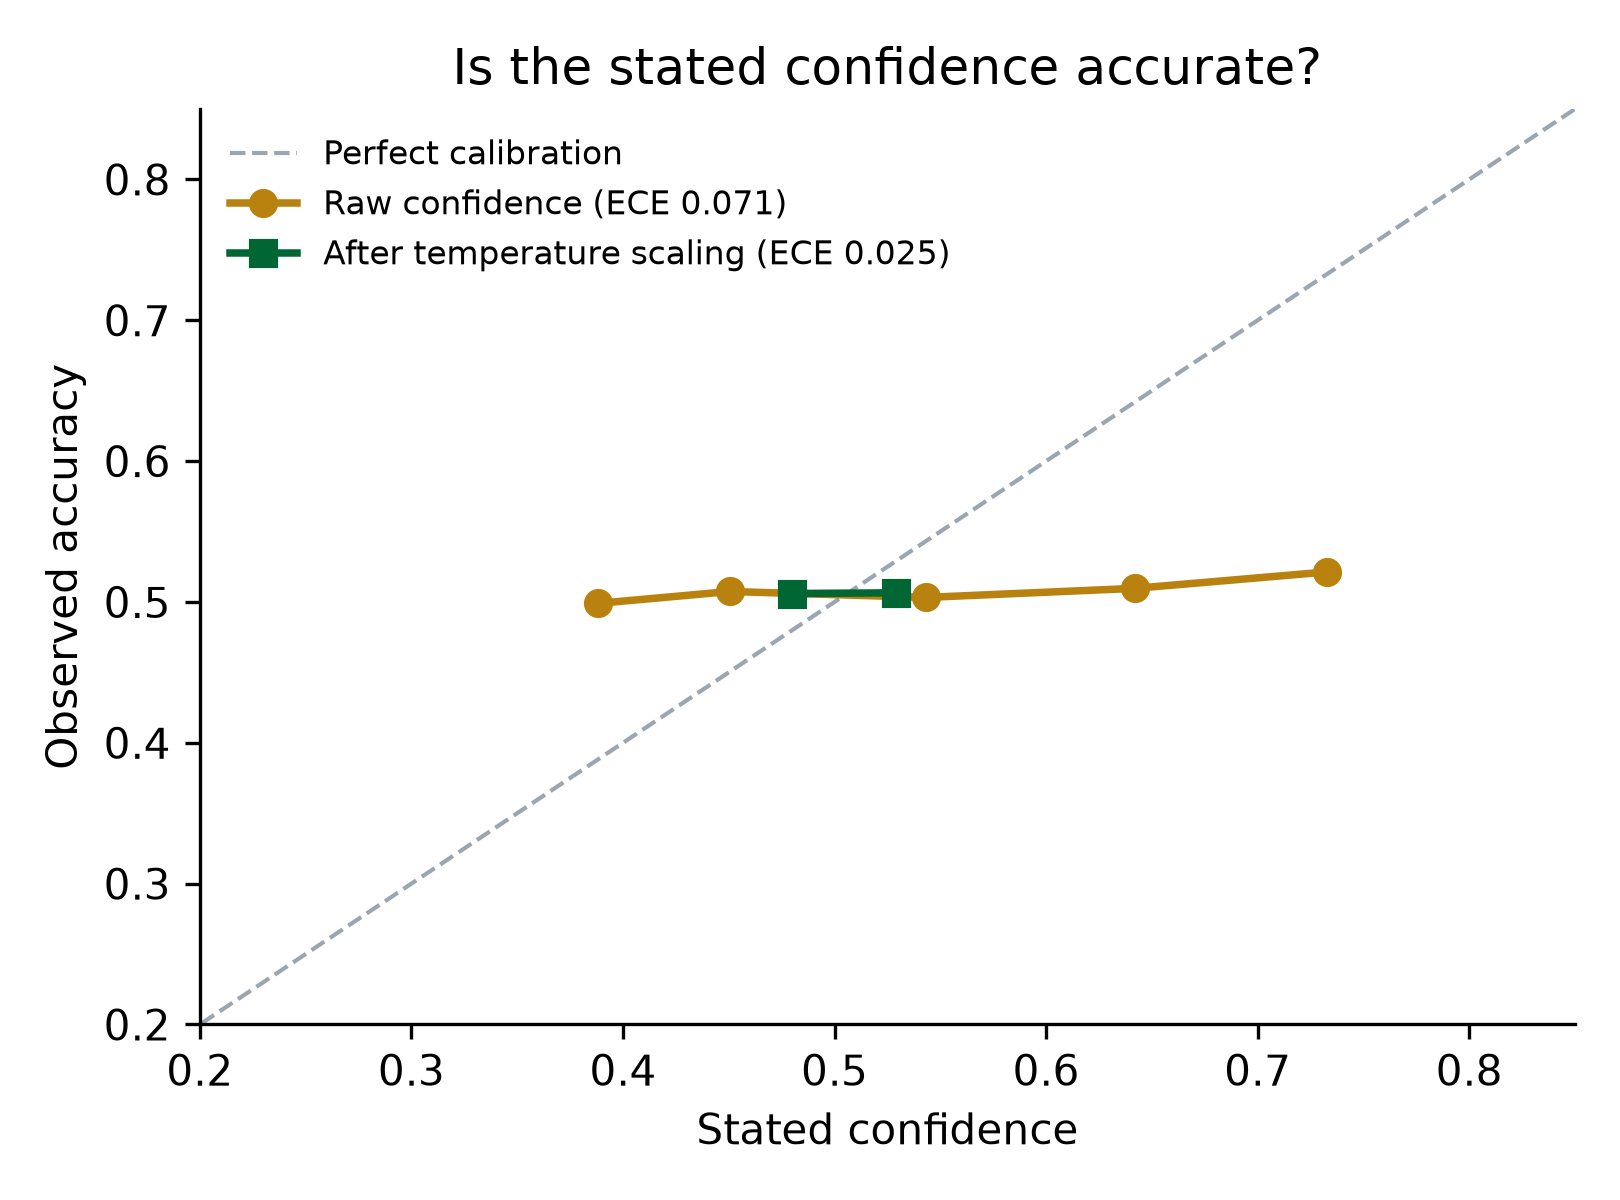
\includegraphics[width=\figW]{figs/fig_reliability.png}
\caption{Reliability of stated confidence for the numeric baseline signal over three years of daily data. Points below the diagonal are over-confident; temperature scaling moves them toward the diagonal.}
\label{fig:rel}
\end{figure}

\begin{figure}[!htbp]
\centering
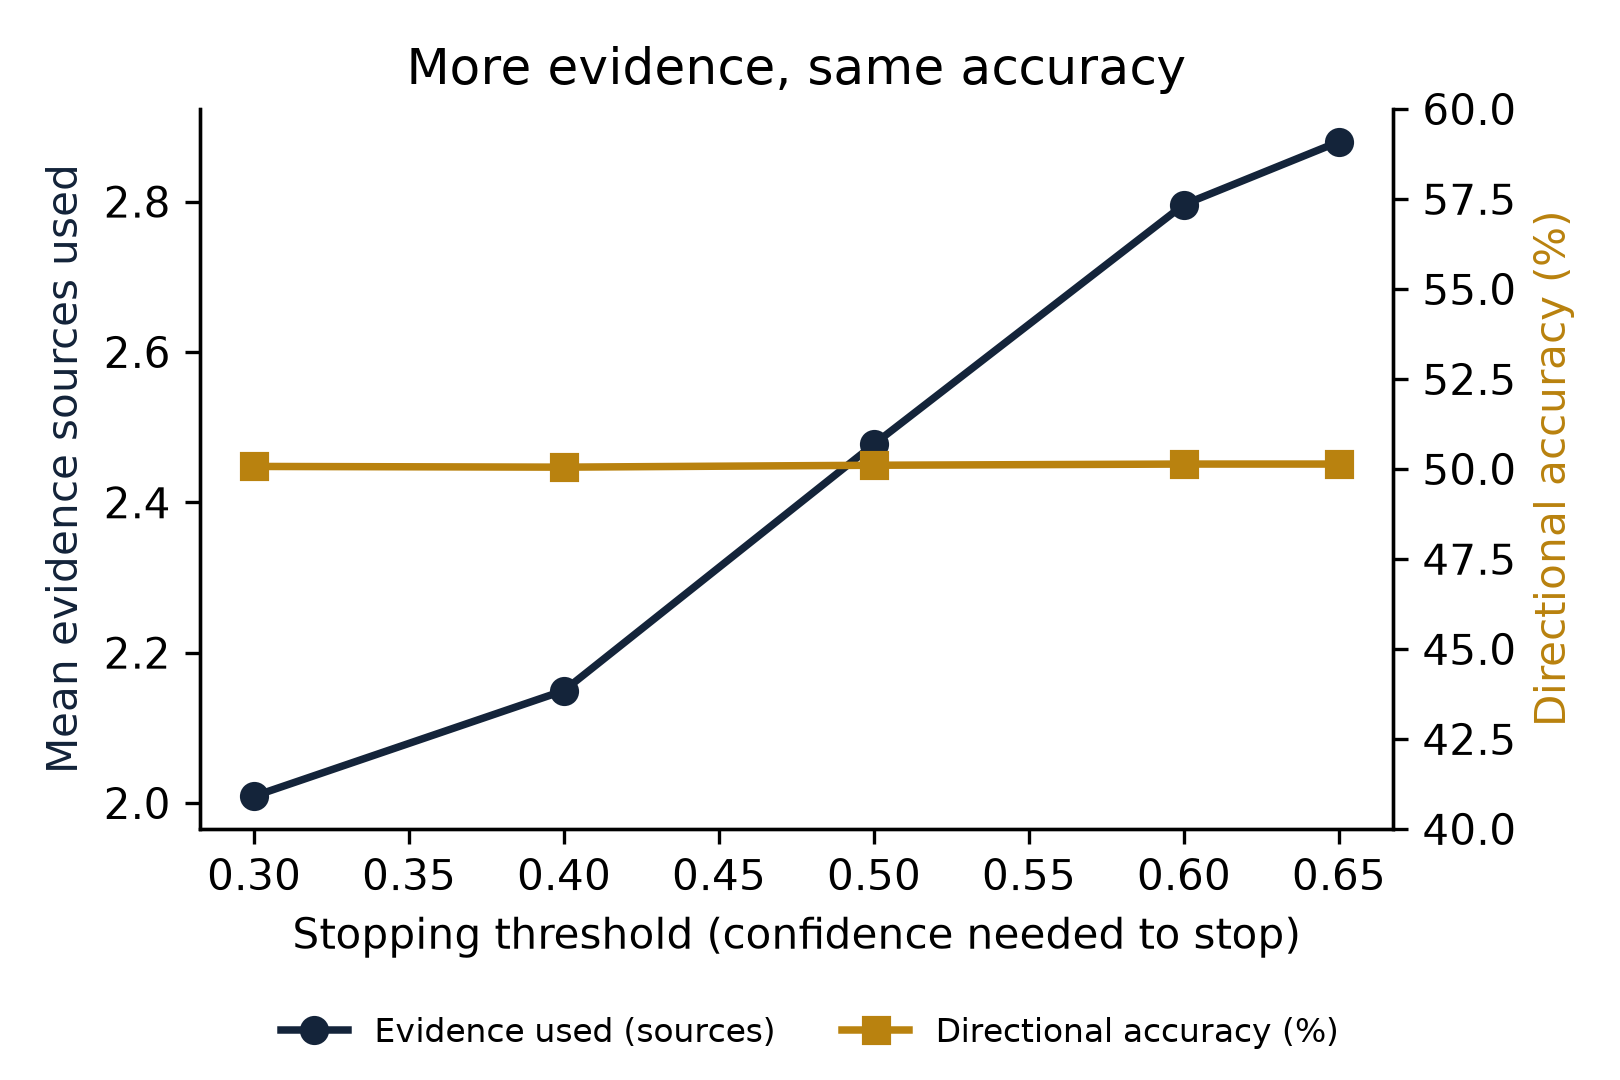
\includegraphics[width=\figW]{figs/fig_cost_quality.png}
\caption{Evidence cost versus directional accuracy as the stopping threshold rises (numeric baseline signals). Cost grows while accuracy stays flat.}
\label{fig:cost}
\end{figure}

\BaselineTable

\subsection{Limitations}
The experiment used one model (\texttt{gpt-4o-mini}), one sample per decision, and evidence from a single day, so it measures rule-following but not the realised outcome of each decision. The numeric baselines cover ten US large-cap stocks, and all trading is simulated. These limits are addressed in the planned work below.

% ---------------------------------------------------------------- 9 conclusion
\section{Conclusion and Future Work}
This work built a policy-conditioned multi-agent trading decision-support system on live US and Indian market data, with a machine-readable investor policy, four LLM agents, risk-based sizing, a deterministic risk engine, and a complete audit trail, together with an evaluation suite that replays identical evidence under different policies. The first experiment shows that an LLM respects explicit numeric limits but does not infer sensible limits from a written investor description, breaking them in about two-thirds of decisions, which the deterministic layer caught. The numeric baselines show no predictive edge and over-confident confidence, a reminder that returns and confidence must be measured rather than assumed.

Planned next steps: (i) measure, decision by decision, whether the risk layer's overrides improve or worsen realised outcomes, following the intervention analysis of Policy-as-Skill \cite{policyasskill}; (ii) replay the LLM agents over post-training-cutoff history to measure their information coefficient and calibration against the numeric baselines; (iii) add deflated-Sharpe and probability-of-backtest-overfitting checks before any performance claim \cite{bailey2014deflated,lopezdeprado2018}; (iv) repeat the experiment across several model families with repeated sampling; (v) run a continuous paper-trading loop on US and NSE stocks; and (vi) release the frozen evidence bundles and scoring scripts.

\section*{Acknowledgment}
The authors thank Dr. P. S. Varade and Dr. Mousami Turuk for their guidance.

\bibliographystyle{IEEEtran}
\bibliography{refs}
